\chapter{Future work}
\label{c:future}

During the course of this project, it became increasingly clear there are some fundamental issues preventing us from exploring the full breadth of what discrete dislocation dynamics has to offer. \href{http://micro.stanford.edu/wiki/M01_How_to_Obtain_and_Run_DDLab}{DDLab} \cite{ddlab}, the code that EasyDD is based on, made some design decisions that ultimately limit its potential. Namely, the lack of attention paid to the cost of dynamic memory allocation, procedural nature of the code, and choice of programming language. These choices were reasonable upon inception, but as the Tarleton group has increased in size and maturity, it has become evident that it is not enough. We are reaching the upper limits of what can be done with \mintinline{matlab}{MATLAB}. There are more things we can do, more things we are doing. But a constant obstacle in obtaining results is how long they take to get and how difficult it is to add new functionality, even changing boundary conditions presents a non-trivial obstacle that requires intimate knowledge of how the finite element mesh is generated.

The work described in \cref{c:easydd,c:topology,c:tractions} has done much in not only producing more accurate simulations, but doing so faster. Fengxian Liu's work on modelling climb, diffusion and inclusions would greatly benefit from better designed code. Haiyang Yu's work on modelling hydrogen \cite{YU2018} and nanoindentation would also stand to benefit a great deal from a parallelised and faster dislocation separation algorithm. Potential work relevant to modelling dislocation dynamics in nuclear reactors such as post-damage cascade dislocation dynamics \cite{sand2014radiation}, necessitates spontaneous generation of dislocations as a network evolves. Including stochasticity in the form of Langevin dynamics \cite{li2019diffusion} is also highly relevant, especially at higher temperatures.

Many of these require a complete overhaul to some of the most fundamental parts of EasyDD. Even so, its potential would be hindered by the fact that \mintinline{matlab}{MATLAB} is a scripting language not designed for scientific computing. It lacks performance, flexibility and many of the modern features that make life easy when dealing with large codebases. Furthermore, the need for licences can represent a prohibitative barrier for users and researchers. Not only this, but the cost of distributed licences that allow \mintinline{matlab}{MATLAB} to run on clusters severely limits scalability and potential for collaboration---something that at one point, inhibited this project.

But there is a better way. Prompted by the public release of the Imperial College COVID-19 source code \href{https://github.com/mrc-ide/covid-sim}{\texttt{https://github.com/mrc-ide/covid-sim}}, and the recurring issues with computational efficiency, compiler compatibility and availability, and fundamental technical debt inherited from \texttt{DDLab} \cite{ddlab}. We started a weekend project that has turned out to be \emph{extremely} promising.

It is our belief that we are currently in a renaissance of programming languages. There are so many exciting modern languages that build and improve upon the lessons of the past. The most promising for scientific computing is widely regarded to be \mintinline{julia}{Julia} \cite{julia}. A paradigm-shifting, open-source JIT (just in time) compiled\footnote{Although as of \texttt{v1.6}, it might be more appropriate to say call \mintinline{julia}{Julia} a JAOT (Just Ahead Of Time) compiled language thanks to its massively improved precompilation capabilities.} language, explicitly designed for scientific computing. It has a number of features that make it an excellent candidate for a new generation of scientific software.
\begin{enumerate}
    \item Multiple dispatch: methods are dispatched and compiled based on the types of their arguments. Types propagate their way through child functions. This lets the compiler generate optimal code for the platform being used.
    \item Type system: its type system is based on set theory, where types are arranged in a genealogical tree with broader types giving way to narrower ones, e.g. \mintinline{julia}{Float64 <: AbstractFloat <: Real <: Number <: Any == true}. Structures can be parametric on type. These features let developers create generic code without bothering with type annotations, and the behaviour will be appropriate for whatever types are used. This kind of code greatly improves modularity and allows for ``magic'' such as automatic differentiation by only defining the basic arithmetic rules for dual numbers. It also allows for zero-cost abstractions, letting users represent mathematical equations as they are written without incurring a performance cost.
    \item CPU and GPU Parallelisation: parallelising loops is trivial. The \href{https://llvm.org/}{\texttt{LLVM}} compiler is platform-agnostic and creates custom, optimal code for almost all CPU and GPU architectures. This means users get platform-specific optimisations for free, and it means the software can remain a single language with no detriment.
    \item Metaprogramming: one of the most powerful and esoteric features of \mintinline{julia}{Julia}. Much like \mintinline{lisp}{Lisp}, code is an object that can be manipulated by the language itself. This allows code to write and modify code. This can be used to autoparallelise functions on different without rewriting. It lets developers precompute values like an extremely powerful C-preprocessor. It even lets developers design custom syntax and perform mathematical transformations on code itself.
    \item Modern features: \mintinline{julia}{Julia} has all the features of a modern programming language. From a booming and quickly growing fully-integrated package ecosystem with standard and registered libraries, some of which are now best in class. Integrated testing and documentation generation systems. Extremely powerful code introspection tools, e.g. one can check type stability, call trees, and different stages of compilation all the way down to machine instructions. Plus it sports all the interactivity and unicode features we have come to expect from modern interpreted languages.
    \item Interoperability: calling other languages from \mintinline{julia}{Julia} is seamless, so the use of external libraries or languages is as easy as calling a \mintinline{julia}{Julia} function. However, \mintinline{julia}{Julia} is so powerful and performant that most of its packages are mono-language. A feature often shared by other modern languages such as \mintinline{go}{Go}, \mintinline{rust}{Rust}, \mintinline{swift}{Swift} and \mintinline{elixir}{Elixir}.
\end{enumerate}

The code can be found here \href{https://github.com/dcelisgarza/DDD.jl}{\texttt{https://github.com/dcelisgarza/DDD.jl}}. Of note are the banners at the top of the README, those point to the documentation; automated, remote testing; test coverage i.e. which lines of code have been hit during testing and how many times; and an interactive Jupyter notebook on Binder. It is the result of the lessons learned while working on EasyDD. Its design avoids the same pitfalls and has a clear vision for usability, modularity, and extensibility, without sacrificing performance.

As this has been a didactic, after hours project to escape the anxieties of the pandemic and resolve the frustrations with some fundamental aspects of EasyDD, it is nowhere near feature complete. Nevertheless, we can provide a small show of current capabilities. For an interactive demo go to the repository and click the Binder banner (rightmost banner) at the top of the README, it will launch an interactive session that runs on the browser.

\section{Next-Gen 3D discrete dislocation dynamics}

As with every simulation, there are parameters that need to be defined. For dislocation plasticity simulations, the number of parameters is quite large, which is why encapsulation (see \cref{ss:encapsulation}) can be so helpful. However, there are also certain relationships between parameters that must be maintained. This is a problem for usability, as it is very easy for one to use non-sensical parameters and be completely unaware of it until a simulation presents unexpected behaviour. We have ``solved'' this issue in EasyDD (see \cref{s:qol}), but it is clunky, unelegant and opaque. Here we solve both issues in a single stroke and offer greater flexibility.

\subsection{Parameter definition}

Setting up simulations is quite easy and there are multiple options.
\begin{enumerate}
    \item Load the data from external files generated by any file extension supported by the \mintinline{julia}{FileIO} ecosystem. In some cases the loaded data has to be used to manually create the structures, but if \mintinline{julia}{JLD2} is used, it works like \mintinline{matlab}{MATLAB}'s \mintinline{matlab}{save()} and \mintinline{matlab}{load()}. JLD2 is advantageous because it saves structure information so loaded variables will be of the correct type, however it is specific to \mintinline{julia}{Julia} and is still under active development.
    \item Use the built-in serialiser. This works like \mintinline{matlab}{MATLAB}'s built-in \mintinline{matlab}{save()} and \mintinline{matlab}{load()} functions. This is another great option that is in-built to the language, but is also \mintinline{julia}{Julia}-specific and successfully reading files is only guaranteed if they were generated with the same version of \mintinline{julia}{Julia} being used.
    \item Use the specially defined functions that load \mintinline{java}{JSON}\footnote{\mintinline{java}{JSON} is an open standard for representing objects as dictionaries in a file. It is widely used by web develpers because it is language agnostic, has high compressibility ratios, and is human-readable.} files and create the structures automatically. Since \mintinline{java}{JSON} is a human-readable format, this is the preferred method for creating sets of parameters that can be used in multiple simulations and loaded from the same file. It is also quite advantageous for sharing data because they have high compressibility ratios and anyone can open a JSON file to have a look at the data. We have internal functions that validate the data and initialise the structures from these files. However, any changes made to the data structures must be accounted for in the IO functions.
    \item Create the structures manually. This can be done by directly using the structure constructors or by using the keyword constructors. When manually creating the variables, using the keyword functions is preferred as they perform validations, calculate derived values, and provide sensible defaults.
\end{enumerate}

Here we show how easy it is to manually set up a simulation. We have to start by defining our parameters.

Almost all of our keyword constructor functions provide default values in case the user does not provide them. They also perform validations on the data to ensure it is sensible, for example the maximum length of a dislocation line must be larger than the minimum length. For demonstration purposes, we provide some values and let the code figure out the rest from what we gave it. This means function signatures can be even shorter than what is shown here.
\begin{minted}[frame=lines, linenos]{julia}
# Dislocation parameters
dlnParams = DislocationParameters(;
    mobility = mobBCC(),
    dragCoeffs = (edge = 1, screw = 1e-1, climb = 1e9, line = 1e-5),
    coreRad = 0.015 * sqrt(2),
    minSegLen = 0.15 * sqrt(2),
    maxSegLen = 1.5 * sqrt(2),
    coreEnergy = 1 / (4 * π) * log(0.015 * sqrt(2) / 3.5e-5),
    coreRadMag = 3.5e-4
)
# Material parameters
matParams = MaterialParameters(;
    crystalStruct = BCC(), μ = 1, μMag = 80e3, ν = 0.25
)
# FEM parameters for a regular cuboid mesh with linear elements
# with the purpose of modelling a cantilever loading experiment
femParamsC = FEMParameters(;
    type = DispatchRegularCuboidMesh(),
    order = LinearElement(),
    model = CantileverLoad(),
    dx = 23.0, # Length in x
    dy = 17.0, # Length in y
    dz = 13.0, # Length in z
    mx = 7, # Elements in x
    my = 5, # Elements in y
    mz = 3  # Elements in z
)
# Slip system information for two BCC slip systems
slipSystems = SlipSystem(;
    crystalStruct = BCC(),
    slipPlane = Float64[-1 1; 1 -1; 0 0],
    bVec = Float64[1 1; 1 1; 1 -1]
)
# Integration parameters
intParams = IntegrationParameters(;
    method = AdaptiveEulerTrapezoid(),
    abstol = dlnParams.collisionDist / 2,
    reltol = dlnParams.collisionDist / 2
)
# Integration time variables
intTime = IntegrationTime(; dt = 0.0, time = 0.0);
\end{minted}
All together, these represent about 60 constants that control all aspects of a simulation. But we're only just getting started.

\mintinline{julia}{Julia} is a fully compiled language, where files can be run from a terminal like any other compiled language. But because it is JIT-compiled, we can ask it questions about our variables, types, functions, etc.\footnote{We represent interactive REPL (Read Eval Print Loop, i.e. \mintinline{julia}{Julia}'s ``terminal''), use by omitting line numbers. Moreover, the \LaTeX{} package, \texttt{minted}, does not accurately represent REPLs so the syntax highlighting will be off in these cases. Regardless, \mintinline{julia}{Julia} uses Markdown natively, so it produces documentation and answers such queries in Markdown-formatted text. Documentation is canonically written as Markdown docstrings (strings of text in Markdown format) within the source, which allows one to browse it interactively. The standard-library documentation package can then be set up to generate HMTL pages and hooked up to a remote testing service which builds and pushes the generated documentation onto the git webhosting service of choice. If using GitHub, one can use ``GitHub Tasks'' to directly build and host documentation there. Other modern languages have similar capabilities.}
\begin{minted}[frame=lines]{julia}
julia>?femParams
search: femParamsC femParamsP FEMParameters loadFEMParameters
  No documentation found.

  femParamsC is of type FEMParameters{DispatchRegularCuboidMesh, 
  LinearElement, CantileverLoad, Float64, Float64, Float64, 
  Int64, Int64, Int64}.

  Summary  
  ========
  struct FEMParameters{DispatchRegularCuboidMesh, LinearElement, 
  CantileverLoad, Float64, Float64, Float64, Int64, Int64, 
  Int64} <: Any

  Fields
  ========
  type  :: DispatchRegularCuboidMesh
  order :: LinearElement
  model :: CantileverLoad
  dx    :: Float64
  dy    :: Float64
  dz    :: Float64
  mx    :: Int64
  my    :: Int64
  mz    :: Int64
\end{minted}

\subsection{Generation of FE mesh and boundary conditions}

With the parameters created, we are now free to build our FE mesh and generate our dislocations. Building and plotting a mesh according to our parameters is simple enough.
\begin{minted}[frame=lines, linenos]{julia}
meshC = buildMesh(matParams, femParamsC)
plotFEDomain(meshC; camera = (10, -2))
\end{minted}
The mesh is built using the canonical numbering system defined in \cite{femcanonical}, and builds the node sets accordingly (shown in \cref{f:feNodeSet}).
\begin{figure}
    \centering
    \includegraphics[width=0.8\linewidth]{feNodeSet.pdf}
    \caption[Canonically defined finite element node sets.]{Canonically defined finite element node sets.}
    \label{f:feNodeSet}
\end{figure}

\mintinline{julia}{Julia} has a parametric type are called, \mintinline{julia}{NamedTuple}.
Which are key-value pairs that can be accessed via indices (as one would a tuple), their keys (as one would a dictionary), or dot syntax (as one would a structure).
\begin{minted}[frame=lines]{julia}
julia> d = (a = 1, b = 2 + im, c = false)
(a = 1, b = 2.0 + 1.0im, false)
julia> d[1]
1
julia> d[b]
2.0 + 1.0im
julia> d.c
false
\end{minted}
They act like on-the fly structures and are very convenient when making composable and generic code. The variable \mintinline{julia}{dlnParams}, keeps the drag coefficients in a \mintinline{julia}{NamedTuple}, which can be accessed through the \mintinline{julia}{dragCoeffs} field. This makes swapping mobility functions a breeze without modifying existing source code. \mintinline{julia}{NamedTuples} are also used in the FE mesh data structure, where they represent surface node sets.
\begin{minted}[frame=lines]{julia}
julia> keys(meshC.surfNode)
(:x0y0z0, :x1y0z0, :x1y1z0, :x0y1z0, :x0y0z1, :x1y0z1, 
 :x1y1z1, :x0y1z1, :x_y0z0, :y_x1z0, :x_y1z0, :y_x0z0, 
 :x_y0z1, :y_x1z1, :x_y1z1, :y_x0z1, :z_x0y0, :z_x1y0, 
 :z_x1y1, :z_x0y1, :xz_y0, :yz_x1, :xz_y1, :yz_x0, 
 :xy_z0, :xy_z1)
\end{minted}
The keys say exactly what they represent, and are canonically ordered \cite{femcanonical}. Corners come first (\mintinline{julia}{:x0y0z0}), then edges (\mintinline{julia}{:x_y0z0}), and finally faces (\mintinline{julia}{:xz_y0}), making the creation of different boundary conditions a very easy, self-documenting, literal process.

We can easily generate the boundary conditions for our model, as well as the sparse vectors that will hold the loading information.
\begin{minted}[frame=lines, linenos]{julia}
# Generate boundary conditions and sparse vectors 
# that will hold loading information
boundaryC, forceDispC = Boundaries(femParamsC, meshC)
# Plot boundary conditions
figCBC = plotBoundaries(boundaryC, meshC)
\end{minted}
This uses our canonical definition of the boundary conditions (\cref{f:cantileverNodeSet}), but users can modify them through keyword arguments.
\begin{figure}
    \centering
    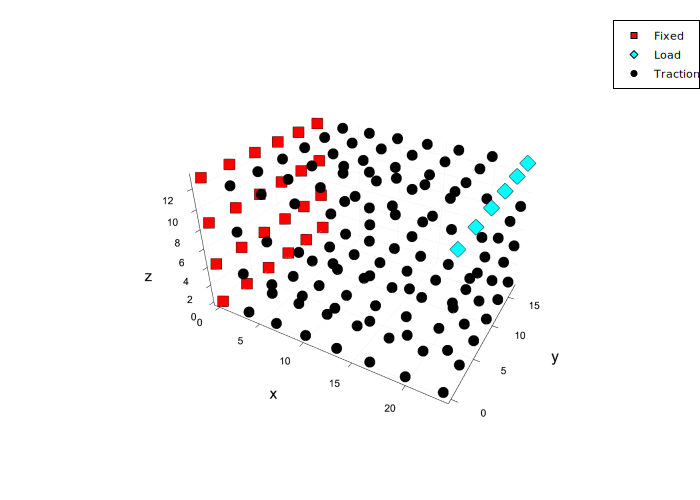
\includegraphics[width=0.6\linewidth]{cantilever.pdf}
    \caption{DDD.jl canonical cantilever loading boundary node sets.}
    \label{f:cantileverNodeSet}
\end{figure}
Through the magic of multiple dispatch, we can also create boundary conditions for pillar loading \cref{f:pillarLoad}. Here we went with a different mesh, but we could just as easily have used the same one as before, as long as the \mintinline{julia}{model} parameter given to the \mintinline{julia}{FEMParameters} is \mintinline{julia}{PillarLoad()}.
\begin{minted}[frame=lines, linenos]{julia}
# Pillar loading
femParamsP = FEMParameters(;
    type = DispatchRegularCuboidMesh(),
    order = LinearElement(),
    model = PillarLoad(),
    dx = 17.0,
    dy = 13.0,
    dz = 23.0,
    mx = 5,
    my = 3,
    mz = 7,
)
meshP = buildMesh(matParams, femParamsP);
boundaryP, forceDispP = Boundaries(femParamsP, meshP);
\end{minted}
\begin{figure}
    \centering
    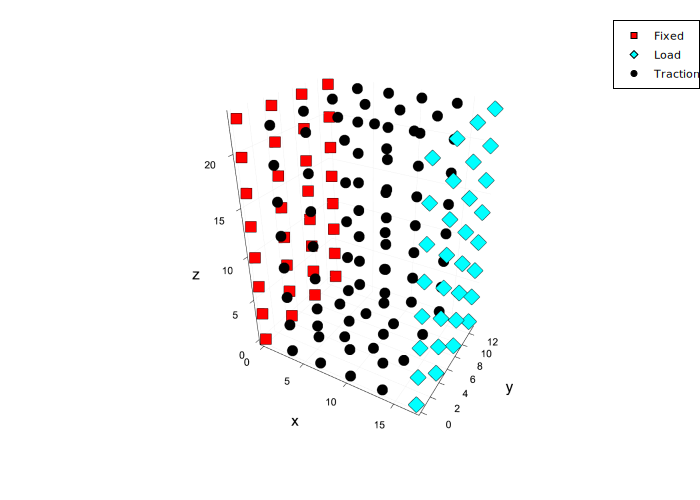
\includegraphics[width=0.6\linewidth]{pillar.pdf}
    \caption{DDD.jl canonical pillar loading boundary node sets.}
    \label{f:pillarLoad}
\end{figure}

\subsection{Generation of dislocation sources}

Generating dislocation sources is also quite easy. We can use some information from the simulation parameters to generate two types of dislocations,
\begin{inparaenum}
    \item prismatic loop with 8 sides, 8 nodes and 8 segments with $\vec{b} = [1\, 1\, 1]$ and $n = [\overline{1}\, 1\, 0]$,
    \item and a shear loop with 5 sides, 10 nodes and 10 segments with $b = [1\, 1\, \overline{1}]$ and $n = [1\, \overline{1}\, 0]$.
\end{inparaenum}
Both structures represent 5 loops with segment lengths of \mintinline{julia}{segLen}, which will be random uniformly distributed $x = [0,\, dx]$, $y = [0,\, dy]$, $z = [0,\, dz]$.
\begin{minted}[frame=lines, linenos]{julia}
# Julia supports multiple assignments in a single line
# Assign the domain size and length scale for the dislocation
# segments.
dx, dy, dz = femParamsC.dx, femParamsC.dy, femParamsC.dz
segLen = (dlnParams.minSegLen + dlnParams.maxSegLen) / 2

prismOct = DislocationLoop(;
    loopType = loopPrism(), # Prismatic loop
    numSides = 8,   # 8 sides
    nodeSide = 1,   # 1 node per side (corners)
    numLoops = 5,   # Will generate 5 loops in the network
    segLen = segLen * ones(8), # Each side is of equal length
    slipSystemIdx = 1,  # Slipsystem 1
    slipSystem = slipSystems,   # Available slip systems
    label = nodeTypeDln.(ones(Int, 8)), # Node type
    buffer = 0, # Spacing for the distribution, may change in the future
    range = [0 dx; 0 dy; 0 dz], # Range on which to distribute
    dist = Rand(),  # Random uniform distribution in space
)
shearPent = DislocationLoop(;
    loopType = loopShear(), # Shear loop
    numSides = 5,
    nodeSide = 2,   # Two nodes per side (corners and mid-segment)
    numLoops = 5,
    segLen = segLen * ones(10), # 10 segments per loop this time
    slipSystemIdx = 2,
    slipSystem = slipSystems,
    label = nodeTypeDln.(ones(Int, 10)),
    buffer = 0,
    range = [0 dx; 0 dy; 0 dz],
    dist = Rand(),
)
\end{minted}
When the loops are generated, only one of each is made, and they are centred about the origin (\cref{f:templateLoops}). Their purpose is to serve as templates for later use.
\begin{figure}
    \centering
    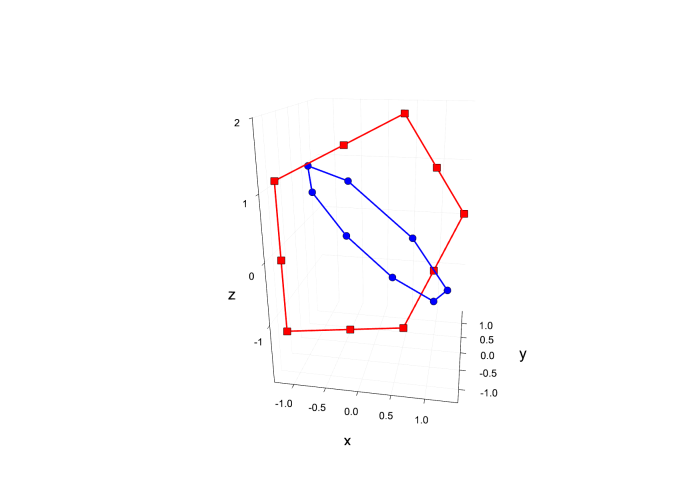
\includegraphics[width=0.6\linewidth]{loops.pdf}
    \caption{Template loops for network generation.}
    \label{f:templateLoops}
\end{figure}

The buffer is defined relative to the average segment length and is only used to space the loops out when calculating their positions from the distribution and range. Currently there are zero, random uniform and random normal distributions, but new ones can be quickly and easily added by subtyping the distribution type and making a function that dispatches on it. The loop generation source code does not have to be modified.

The type \mintinline{julia}{nodeTypeDln} only has a limited number of values, each of them with a specific meaning. This provides a safeguard against regressions and useful information to users and developers. For example, by looking at the loop's labels we see that they are \mintinline{julia}{intMobDln}, i.e. internal mobile dislocation nodes. Each node type behaves differently and the values are limited to the types of nodes the code supports. A similar technique is used to denote node sets on the finite element side.
\begin{minted}[frame=lines, linenos]{julia}
julia> prismOct.label
8-element Array{nodeTypeDln,1}:
 intMobDln::nodeTypeDln = 1
 intMobDln::nodeTypeDln = 1
 intMobDln::nodeTypeDln = 1
 intMobDln::nodeTypeDln = 1
 intMobDln::nodeTypeDln = 1
 intMobDln::nodeTypeDln = 1
 intMobDln::nodeTypeDln = 1
 intMobDln::nodeTypeDln = 1
\end{minted}

We can visualise the loop using a myriad of plotting backends but we will use an interactive one similar to \mintinline{matlab}{MATLAB}'s\footnote{\mintinline{matlab}{MATLAB} uses a modified version of this backend.}
\begin{figure}
    \centering
    \includegraphics[trim={5cm 1cm 5cm 3cm},clip,width=0.5\linewidth]{prismOct.pdf}
    \caption[Sample 8-sided prismatic BCC dislocation loop.]{Sample 8-sided prismatic BCC dislocation loop with slip plane $ \vec{n} = [\overline{1}\, 1\, 0] $, and Burgers vector $\vec{b} = [1\, 1\, 1]$.}
\end{figure}

\begin{minted}[frame=lines, linenos]{julia}
using Plots
plotlyjs()

fig = plotNodes(
    prismOct,
    m = 1,
    l = 3,
    linecolor = :blue,
    marker = :circle,
    markercolor = :blue,
    legend = false,
)
\end{minted}

We can create a prismatic loop in the same way by changing the \mintinline{julia}{loopType} to the shear type, and visualise in the same space by mutating\footnote{By convention, functions that mutate their arguments are denoted by adding an \texttt{!} at the end of the function name.} the figure. This time we will create 10 and distribute them random normally in the domain.
\begin{figure}
    \centering
    \includegraphics[trim={5cm 1cm 5cm 3cm},clip,width=0.5\linewidth]{shearOct.pdf}
    \caption[Sample 8-sided shear prismatic BCC dislocation loop.]{Adding 10, 8-sided shear BCC dislocation loop with slip plane $ \vec{n} = [\overline{1}\, 1\, 0] $, and Burgers vector $\vec{b} = [1\, 1\, 1]$.}
\end{figure}
\begin{minted}[frame=lines, linenos]{julia}
shearOct = DislocationLoop(;
    loopType = loopShear(),
    numSides = 8,
    nodeSide = 1,
    numLoops = 10,
    segLen = segLen * ones(8),
    slipSystemIdx = 1,
    slipSystem = slipSystems,
    label = nodeTypeDln.(ones(Int, 8)),
    buffer = 0,
    range = [
                0 dx; 
                0 dy;
                0 dz
            ],
    dist = Rand(),
)
plotNodes!(
    fig,
    shearOct,
    m = 1,
    l = 3,
    linecolor = :red,
    marker = :circle,
    markercolor = :red,
    legend = false,
)
\end{minted}
As both loops have the same BCC slip system, they are orthogonal to one another.

The \mintinline{julia}{DislocationLoop} structure only denotes dislocation loops, it does not represent the network. The number of loops in the structure, \mintinline{julia}{numLoops}, is what determines how many will be generated. The values of \mintinline{julia}{buffer}, \mintinline{julia}{range} and \mintinline{julia}{dist} determine how they are distributed.

Dislocation networks can be generated manually by specifying all their relevant fields, giving flexibility for the generation of bespoke networks or by using the \mintinline{julia}{DislocationLoop} structure. The latter is easier and more convenient. If certain types of bespoke structures, such as mixed-slip system loops, jogs or kinks, it would be prudent to utilise multiple dispatch and define a specific \mintinline{julia}{DislocationLoop()} function for the purpose. Making the network is quick and painless. There are also default arguments that change things such as how much memory to allocate to allow for the network to expand and the maximum number of connections a node in the network is allowed to have. The default is to allocate $N\log_2N$ places for $N$ total nodes and segments in the network. The topological operations also use this heuristic when the network needs to be expanded further.
\begin{minted}[frame=lines, linenos]{julia}
network = DislocationNetwork([prismOct, shearOct])
\end{minted}

We could view the network like this, but where's the fun in that? We'll first generate the mesh. And while we're at it we can make the boundary conditions according to \mintinline{julia}{matParams} and \mintinline{julia}{femParams}. We specified in the creation of \mintinline{julia}{femParams} that we would like to model a \mintinline{julia}{CantileverLoad()} dispatching on a \mintinline{julia}{DispatchRegularCuboidMesh()} with elements of order \mintinline{julia}{LinearElement()}. All this ensures the mesh is built of the correct order and type. Adding mesh types only requires the definition of the appropriate types and the mesh generation function. Users do not need to worry about calling different functions.
\begin{minted}[frame=lines, linenos]{julia}
regularCuboidMesh = buildMesh(matParams, femParams)
cantileverBC, forceDisplacement = Boundaries(
                                    femParams, 
                                    regularCuboidMesh
                                )
\end{minted}
In \cref{f:feNodeSet} we can visualise the node sets generated by \mintinline{julia}{buildMesh()}. These are used to very easily generate the boundary conditions without knowing the details of how the FE mesh builder works. This greatly expedites the process of defining the boundary conditions for different scenarios. They define which finite element nodes belong to corners, edges and faces. Those not labelled are internal. These are all generated by the mesh builder and is a requirement that forces developers to make the sensible decision of creating node sets so their work is usable by others simply by looking at which nodes belong to which set.

\begin{minted}[frame=lines, linenos]{julia}
plotFEDomain(regularCuboidMesh)
\end{minted}

Now that we have our FE mesh and network we can see what they look like.
\begin{figure}
    \centering
    \includegraphics[trim={5cm 0cm 5cm 1.5cm},clip,width=0.5\linewidth]{sampleDomain.pdf}
    \caption[Sample network and domain.]{Dislocation network and domain.}
\end{figure}
\begin{minted}[frame=lines, linenos]{julia}
plotNodes(
    regularCuboidMesh,
    network,
    m = 1,
    l = 3,
    linecolor = :blue,
    marker = :circle,
    markercolor = :blue,
    legend = false,
)
\end{minted}

Since we decided to randomly distribute 10 relatively large loops in the domain, there are some segments that are poking out. We can fix that by using the surface remeshing. However, the function requires nodal velocities to work because we need a vector to define the intersection with the surface of the volume.

As of the time of writing, the surface remeshing has not been thoroughly tested and the currently implemented mobility function is out-dated. So instead, we use a random velocity as a stand-in for the real and updated velocities. However, this surface remeshing works for any convex hull regardless of mesh type. It also does not require a surface tasselation because defining the convex hull (using the vertices and a \mintinline{julia}{JuliaGeometry} library), surface normals, and mid-points is enough to exactly determine how to project external nodes. Moreover, the value used to decide how far the nodes should be projected is not hard-coded and is in fact the scale of the FE domain ($\sqrt[3]{\Delta x \Delta y \Delta z}$), ensuring there is always an appropriate closure point for calculating dislocation displacements no matter the domain's aspect ratio.
\begin{minted}[frame=lines, linenos]{julia}
numSeg = network.numSeg[1]
network.nodeVel[:, 1:numSeg] = rand(3, numSeg)
network = remeshSurfaceNetwork!(regularCuboidMesh,  network)
\end{minted}
This showcases one of the quirks of immutable structures in \mintinline{julia}{julia}. Immutable structures are faster and more easily optimised. But arrays inside them cannot be expanded and the values of non-array fields cannot be changed. However, the values of elements inside arrays can be changed. So to keep track of the number of nodes and segments they are vectors of length 1. Also, any function with the potential for resizing the arrays of an immutable structure, has to return the structure, else the new array entries get lost and garbage collected later. Since \mintinline{julia}{remeshSurfaceNetwork!()} can change the values inside the arrays of \mintinline{julia}{network} as well as resize them, its return value gets reassigned to \mintinline{julia}{network}. After running this we get a properly internal network with a bunch of surface nodes.
\begin{figure}
    \centering
    \includegraphics[trim={5cm 0cm 5cm 1.5cm},clip,width=0.5\linewidth]{remeshedSurf.pdf}
    \caption[Sample network and domain with remeshed surface.]{Sample network and domain with remeshed surface.}
\end{figure}

As previously stated, this has been mostly a didactic exercise. However, as of the time of writing, the code has the following capabilities.
\begin{enumerate}
    \item IO,
    \item loop and network generation,
    \item regular cuboid mesh generation,
    \item boundary conditions for cantilever bending,
    \item internal remeshing,
    \item surface remeshing,
    \item dislocation displacements,
    \item forces on segments,
    \item field point stresses,
    \item outdated BCC mobility function,
    \item time integration.
\end{enumerate}

All of which are faster than what is offered by EasyDD---even those accelerated by \mintinline{c}{C}. The $\mathcal{O}(N^2)$ segment-segment calculation is 10\% faster than its equivalent \mintinline{c}{C} function and has already been CPU-parallelised; for large numbers of dislocations it offers linear scaling with number of threads. The self-forces and Peach-K\"{o}hler forces as a result of the dislocations being inside a cuboid mesh are both $10\times$ faster than their \mintinline{matlab}{MATLAB} counterparts. Since the mesh refinement uses a better heuristic than dynamically sizing arrays every time a new node is added to the network, it is about as slow as \mintinline{matlab}{MATLAB}'s when it needs to allocate memory, but when it does not it is $>100\times$ faster. Mesh coarsening is $3\times$ faster. The calculation of field point stresses for numeric tractions is $30\%$ faster than its \mintinline{c}{C} counterpart. Building the FE mesh is $>10\times$ faster. The outdated mobility law is $>30\times$ faster and in all the tests has not required dampening the matrix inversion. The dislocation displacement calculation is $>10\times$ faster. The cholesky factorisation is $20\times$ faster and uses a substantially smaller amount of memory.

The memory footprint is also \emph{a lot} lower. Care has been taken to do things as optimally as possible and \mintinline{julia}{Julia}'s typesystem lets sparse arrays be treated in \emph{exactly} the same way as dense ones, which is not always the case in \mintinline{matlab}{MATLAB}, which has thwarted efforts at sparsifying various arrays that would benefit from it.

The total number of lines of code so far, $\sim 3200$ are the equivalent of $\sim 4500$ \emph{without} counting input files and the many different loop generation functions. However this accounts for mutating and non-mutating functions, which are essentially the same implementation only non mutating functions allocate a return value while mutating ones change their arguments. Mutating functions tend to be faster because of the lack of heap allocation, but we decided to make both as only the indexing changes. Accounting only for single versions of mutating or non-mutating functions yields $\sim 1800$ unique lines of code, which is about the same number of lines in the segment-segment \mintinline{c}{C} function.

Moreover, doing the equivalent of what we have shown on EasyDD requires a substantially larger amount of code and a not insignificant amount of knowledge of its inner workings. From generating the network, to defining values for its parameters---which, despite the fact that EasyDD provides a reasonable set of defaults, users can easily define derived parameters incorrectly and be none the wiser. The barrier to entry and potential for error are quite high. Even us, who use the code all the time and have worked on it, sometimes miss things only to catch them after a simulation does something unexpected.

The one knock on \mintinline{julia}{Julia} is its JIT-compiled nature. Which leads to a notoriously long time to first plot and means functions are slow the first time they are run during a session because they need to be compiled. However this is quickly improving and can be solved by keeping a precompiled system image of the offending packages. There is also the conspicuously poor performance of the \texttt{spy()} function, even with the \mintinline{julia}{UnicodePlots} backend. Having said that, the power, flexibility and ease of use of \mintinline{julia}{Julia} greatly outweighs such small issues.

\section{Conclusions and proposal}\label{s:concProp}

What started as a side project to learn and escape from the world during the last year has resulted in quite a promising avenue for future research. One that lets us have our cake and eat it too. Not only is it performant, it is almost trivially parallelisable on both CPUs and GPUs; while staying easy to use and develop. What \mintinline{julia}{Julia} offers is almost incomprehensible. The performance of \mintinline{c}{C} and \mintinline{fortran}{Fortran}; the syntax and interactivity of \mintinline{python}{Python} and \mintinline{r}{R}; metaprogramming of \mintinline{lisp}{Lisp}; and fully integrated testing and package environments of \mintinline{rust}{Rust} and \mintinline{go}{Go}.

A tool is only as good as the craftsman who weilds it. We aspire to be among those elite craftsmen. Why then, should we not use as good a tool as we can? During the course of this project, the whole Tarleton group have made gigantic strides with EasyDD. It has indeed come a \emph{very} long way, but we can do better.

Some issues are so deeply intertwined with how the software was originally designed that they cannot be separated from how it fundamentally operates. To fix them, a fresh new start is needed. Given the extremely encouraging results of what amounts to a pandemic hobby, we think it worthwhile to continue this as a research software engineering project post-DPhil. We think it is better to do so now rather than wait until there is no more juice left to squeeze out of \mintinline{matlab}{MATLAB}. Not only so the shackles of proprietary software can be broken; but also so the full, ambitious vision of EasyDD can be realised.
% 3644 words
